\documentclass{sem5}
\institutename{Indian Institute of Information Technology, Vadodara}
\author{Dilip Puri}
\idt{201351014}
%\team{teamname}
\collab{\textbf{Collaborator} - Hemant Kumar(201352026)}

\coursename{Parallel Programming}
\ccode{\begin{small}CS403\end{small}}
\profname{Prof. Reshmi Mitra}

\type{Lab}
\typeid{02}
\submissiondate{\today}%dd/mm/yyyy
\deadline{Aug 26, 4:00 PM}%dd/mm/yyyy @hh:mm pm/am
\problemset{Mutex, Conditional Variable, Producer-consumer}

\begin{document}
\begin{enumerate}
\item Familiarize yourself with rw$\_$lock and barrier code in the sample code folder. Run the code and attach the screen-shots with your observations.
\begin{figure}[!htp]
\centering
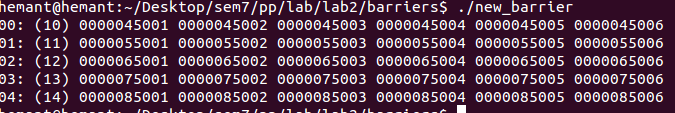
\includegraphics[scale=.4]{../barrier.png}\\
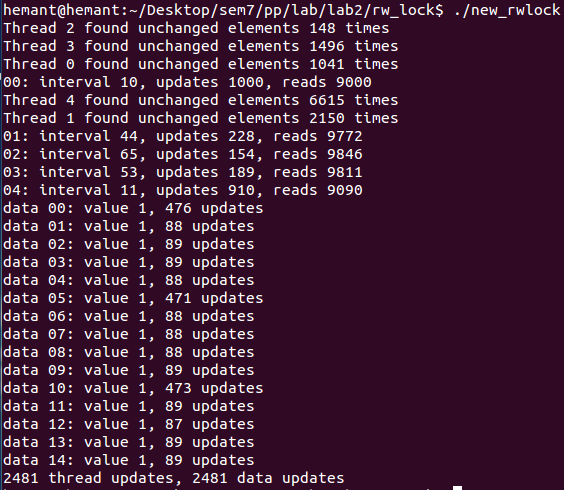
\includegraphics[scale=.4]{../rwlock.png}
\end{figure}
\item For the given serial code (dotprod.c in the sample code folder), write the equivalent parallel code. Using the time command, measure the execution time and corresponding speed-ups for:\\
\begin{itemize}
\item vector length = 100,000 and 200,000
\item number of processors = 2, 4 and 8
\end{itemize}
\begin{center}
\begin{tabular}{|c|c|c|c|c|}
\hline
& p=1 & p=2 & p=4 & p=8\\
\hline
Vector Length = 100,000 & 0.0095 & 0.0124 & 0.0121 & 0.0102 \\
\hline
Vector Length = 200,000 & 0.014 & 0.0166 & 0.0121 & 0.0163 \\
\hline
\end{tabular}

\end{center}
\end{enumerate}
\begin{center}
$Speedup = \frac{Execution Time(p)}{Execution Time(serial code)}$\\
\vspace*{1cm}
\begin{tabular}{|c|c|c|c|}
\hline
 & p=2 & p=4 & p=8\\
\hline
Vector Length = 100,000 & 1.31 & 1.27 & 1.07 \\
\hline
Vector Length = 200,000 & 1.19 & 1.26 & 1.16 \\
\hline
\end{tabular}
\end{center}
\begin{itemize}
\item[3] Multi-access threaded queue
\begin{enumerate}
\item Implement a multi-access threaded queue with multiple threads inserting and multiple threads extracting from the queue. Use mutex-locks to synchronize access to this queue. Document the time for 1000 insertion and 1000 extractions each with 4 insertion threads (producers) and 4 extraction threads (consumers).

\item Repeat above problem with condition variables (in addition to mutex locks). Document the time for the same test case as above. Comment on the difference in the times.

\end{enumerate}
\end{itemize}
\end{document}